%% Hand-maintained from Table~\ref{tab:main} (TUNED rows). The earlier
%% three-panel version plotted clairvoyant energy and start columns taken from
%% the superseded results file; Table~\ref{tab:main} omits those columns, so
%% they are not plotted here either.
\begin{figure}[t]
\centering
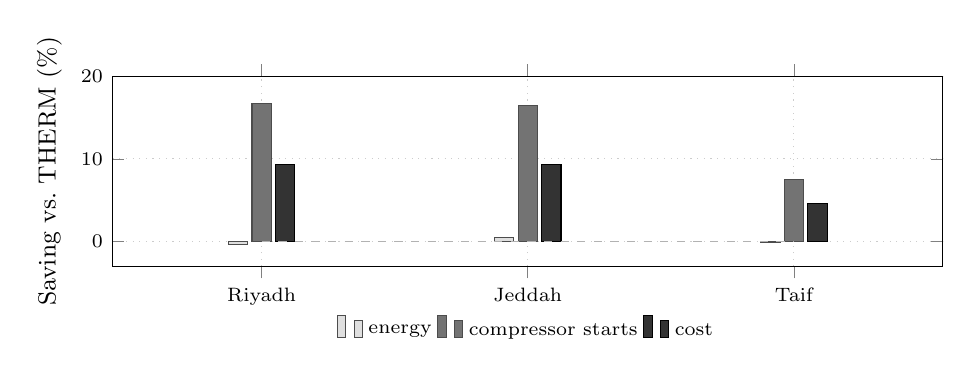
\begin{tikzpicture}
\begin{axis}[
  width=\columnwidth, height=4.0cm,
  ybar=1.5pt,
  bar width=7pt,
  grid=major, grid style={dotted,gray!40},
  tick label style={font=\scriptsize},
  label style={font=\small},
  ylabel={Saving vs.\ THERM (\%)},
  symbolic x coords={Riyadh,Jeddah,Taif},
  xtick=data,
  ymin=-3, ymax=20,
  enlarge x limits=0.28,
  legend style={at={(0.5,-0.22)},anchor=north,legend columns=3,
                font=\scriptsize,draw=none,fill=none},
]
\addplot+[draw=black!70,fill=gray!25]
  coordinates{(Riyadh,-0.3)(Jeddah,0.5)(Taif,-0.1)};
\addlegendentry{energy}
\addplot+[draw=black!70,fill=black!55]
  coordinates{(Riyadh,16.7)(Jeddah,16.4)(Taif,7.5)};
\addlegendentry{compressor starts}
\addplot+[draw=black,fill=black!80]
  coordinates{(Riyadh,9.3)(Jeddah,9.3)(Taif,4.6)};
\addlegendentry{cost}
\draw[gray!60,dashed] (axis cs:Riyadh,0) -- (axis cs:Taif,0);
\end{axis}
\end{tikzpicture}
\caption{The saving is a switching saving. For the tuned rule, the arm whose
energy and start columns Table~\ref{tab:main} reports in full, energy moves by
less than one point in either direction while compressor starts fall by $7.5$
to $16.7\%$ and cost by $4.6$ to $9.3\%$. Identity~\eqref{eq:duty_identity}
requires exactly this once mean occupied temperatures are matched: with the
mean fixed, the duty cycle and hence the energy are fixed too, and what is left
to recover is the per-start charge. Source:
Table~\ref{tab:main}.}
\label{fig:decomp}
\end{figure}
